\subsection{Anotações\label{sec:anotacoes}}
Conforme acordado, a primeira solução a ser implementada no sentido de auxiliar no processo de sistematização das contribuições será baseado na ferramenta \href{http://hypothes.is}{\textit{Hypothes.is}}%
\footnote{\textit{Hypothes.is} - \url{http://hypothes.is} - ``\textit{Nossa missão é trazer uma nova camda para a web. Utilize o Hypothes.is para debater, colaborar, organizar sua pesquisa ou fazer anotações pessoais.}'' (tradução própria) - Acessado em 10/04/2015}.

De forma geral, o que esta ferramenta propõe é adicionar uma nova camada a um website que permita a realização de anotações em quaisquer trechos de texto. Uma analogia possível seria a utilização de um papel vegetal sobre um documento para que se possa realizar anotações no documento sem modificá-lo.

Ao selecionar um trecho de texto, a ferramenta apresenta duas opções, conforme apresentado na Figura \ref{fig:hypotesis-opcoes}. O usuário pode adicionar um comentário (\textit{note}) relativo ao trecho selecionado ou apenas destacar o trecho de texto (\textit{highlight}).

    \begin{figure}[htb]%
        \begin{center}
            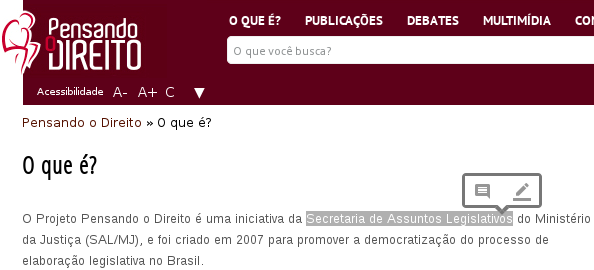
\includegraphics[scale=0.7]{./imagens/hypotesis-opcoes.png}%
        \end{center}%
        \caption{Opções da ferramenta Hypotes.is ao selecionar um texto\label{fig:hypotesis-opcoes}}%
        \fonte{Autoria Própria}%
    \end{figure}%
    
Na Figura \ref{fig:hypotesis-highlight}, podemos observar um parágrafo no qual foi utilizado o recurso de destaque (\textit{highlight}). Nele pode-se perceber alguns trechos que receberam mais de um destaque e, por conta disto, apresentam-se grifados numa coloração mais escura decorrente, desta sobreposição de grifos. O mesmo valeria caso os trechos em questão tivessem sido comentados, eles também receberiam o grifo de destaque, que pode ser sobreposto escuracendo o trecho. Assim, trechos com grifos mais escuros representam trechos mais comentados, ou seja, trechos que receberam mais atenção.

    \begin{figure}[htb]%
        \begin{center}
            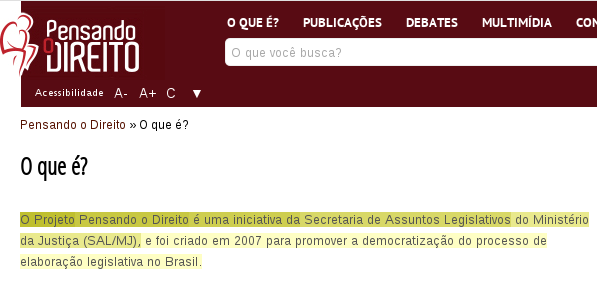
\includegraphics[scale=0.7]{./imagens/hypotesis-highlight.png}%
        \end{center}%
        \caption{Destaques sobrepostos nos textos\label{fig:hypotesis-highlight}}%
        \fonte{Autoria Própria}%
    \end{figure}%

Na Figura \ref{fig:hypotesis-trechos-destacados} podemos observar a barra lateral da ferramenta. Nela estão os trechos que foram selecionados e destacados, assim como também estão trechos que foram comentados. Ainda existe a opção para buscar comentários que tenham determinados termos e a opção de ordenar os comentários e destaques por ordem de criação - do mais antigo para o mais novo e do mais novo para o mais antigo; além da ordenação por ``localização'', na qual os comentários são mostrados ordenados de acordo com a ordem de ocorrência do trecho ao qual o comentário se refere. 
\begin{landscape}
    \begin{figure}[htb]%
        \begin{center}
            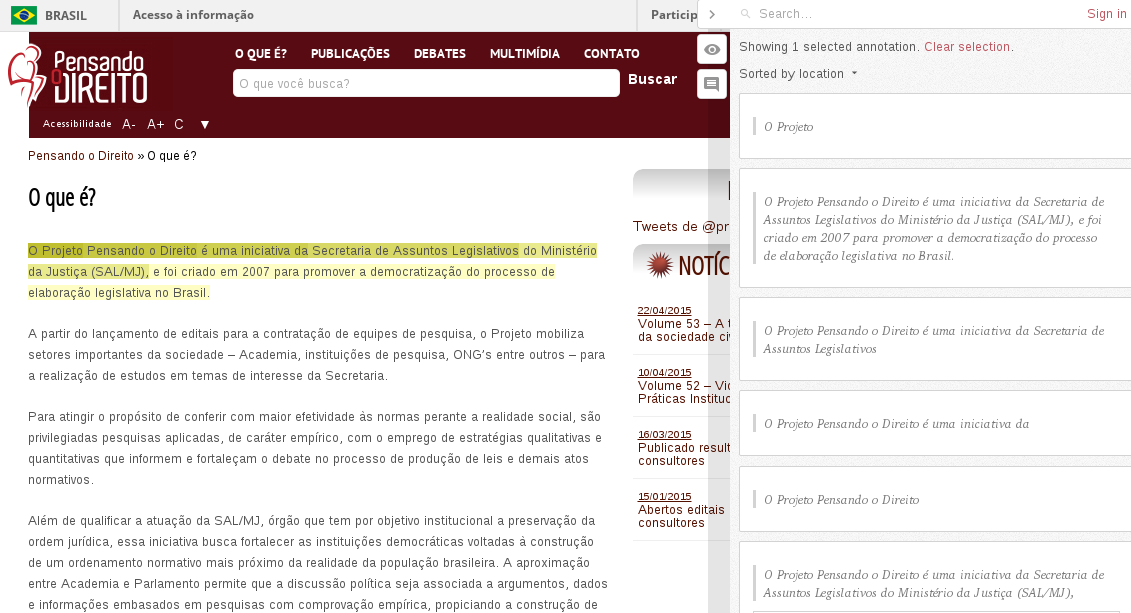
\includegraphics[scale=0.55]{./imagens/hypotesis-trechos-destacados.png}%
        \end{center}%
        \caption{Lista de trechos de texto destacados\label{fig:hypotesis-trechos-destacados}}%
        \fonte{Autoria Própria}%
    \end{figure}%
\end{landscape}
\begin{landscape}
Além da possibilidade de simples destaque, a ferramenta também permite comentários atrelados a trechos de texto selecionados. Estes comentários podem ainda receber \textit{tags}, e sobre eles podem haver outros comentários, permitindo assim algum tipo de debate/discussão. Na Figura \ref{fig:hypotesis-comentario} podemos observer um comentário relativo a um destaque no texto e as tags marcadas no comentário. Além disso, pode-se perceber também que elementos, como um vídeo, também podem receber comentários.

    \begin{figure}[htb]%
        \begin{center}
            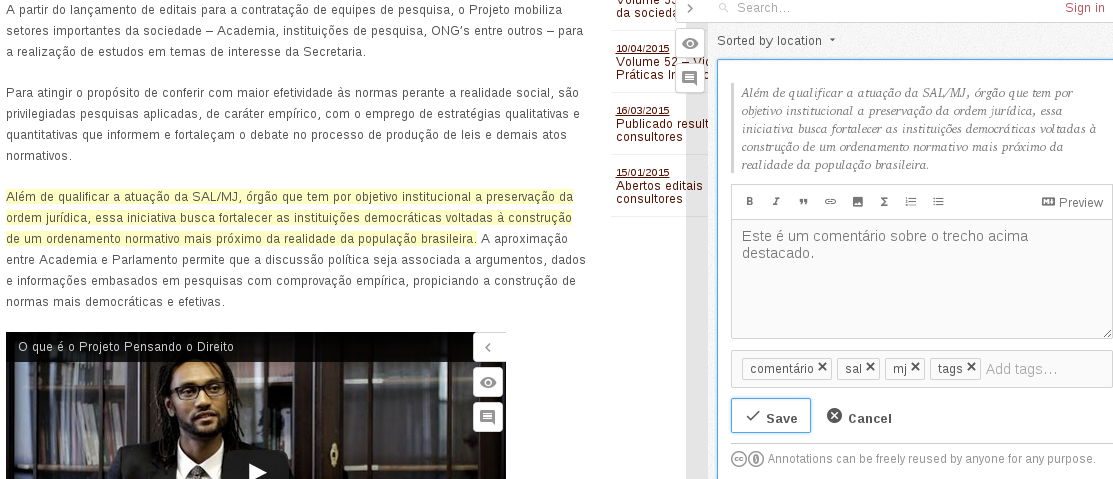
\includegraphics[scale=0.55]{./imagens/hypotesis-comentario.png}%
        \end{center}%
        \caption{Lista de trechos de texto destacados\label{fig:hypotesis-comentario}}%
        \fonte{Autoria Própria}%
    \end{figure}%
\end{landscape}

